\begin{figure*}[tb]
	\centering
	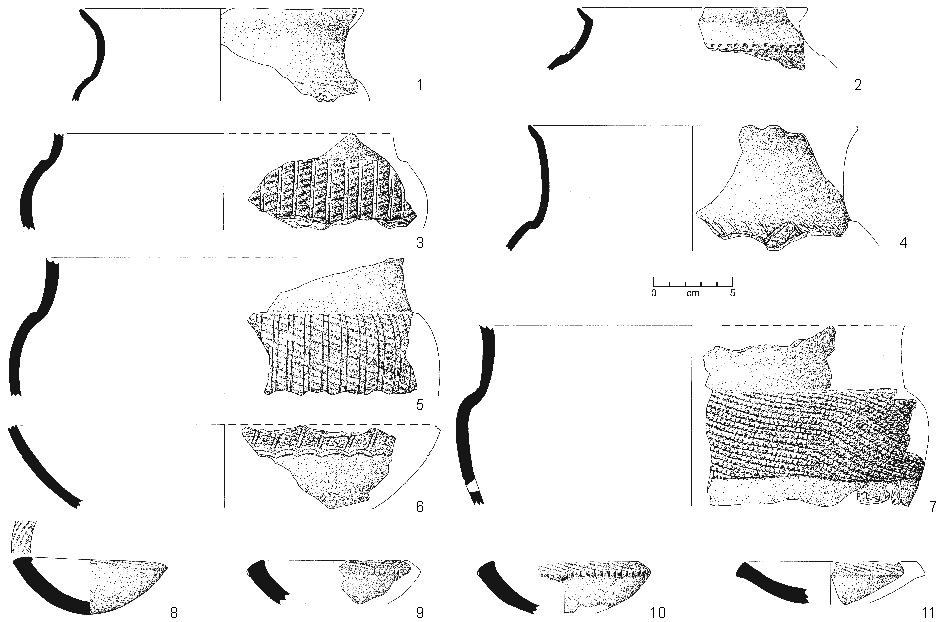
\includegraphics[width=\textwidth]{fig/PDM-Typen.pdf}
	\caption{Pandama-Gruppe: Typvertreter.\\1:~Taf.~63.15; 2:~Taf.~63.18; 3:~Taf.~66.6; 4:~Taf.~63.17; 5:~Taf.~64.1; 6:~Taf.~64.9; 7:~58.4.; 8:~Taf.~63.20; 9:~Taf.~61.11; 10:~Taf.~61.10; 11:~Taf.~61.13.}
	\label{fig:PDM_Typvertreter}
\end{figure*}

\subsubsection{Pandama-Gruppe}\label{sec:PDM-Gr}

An 24 Fundstellen, ausschließlich am mittleren und oberen \mbox{Sangha} sowie dem prospektierten Abschnitt des \mbox{Ngoko}, wurde eine weitere keramische Stilgruppe beobachtet, deren vorwiegend rundbauchige Gefäße regelhaft mit \textit{knotted strip}-Roulette in Kombination mit vertikalen oder diagonalen Riefen verziert sind (Abb.~\ref{fig:PDM_Typvertreter}). Das Fundgut der Pandama-Gruppe umfasst fast ausschließlich isolierte Wandungsscherben (81\,\%), die vor allem anhand der genannten Verzierung dieser Gruppe zugewiesen werden. Lediglich drei nahezu vollständige Gefäße, die 0,5\,\% aller GE der Pandama-Gruppe ausmachen, konnten im Material identifiziert werden. GE sind grundsätzlich stark fragmentiert und 80\,\% aller Stücke sind kleiner als 70$\times$70\,mm. Während bezogen auf die Anzahl an GE die gleiche Anzahl Stücke aus Grabungen (49,5\,\%) wie auch von Oberflächenabsammlungen (50,5\,\%) stammt, unterscheidet sich diese Verteilung bei Betrachtung des Scherbengewichts deutlich. Das aus den beiden in Pikunda am \mbox{Sangha} (Fpl.~255) ausgegrabenen Gruben PIK~87/1 (Kat.-Nr.~8) sowie PIK~87/2 (Kat.-Nr.~9) stammende Fundmaterial, das einzige aus ergrabenem Kontext, zeigt eine deutlich stärkere Fragmentierung und macht lediglich 20\,\% aller GE der Pandama-Gruppe aus. Das Gros der Funde aus Oberflächenabsammlungen stammt vom namensgebenden Fundplatz Pandama am \mbox{Ngoko} (Fpl.~276). Die Oberflächenfunde dieses Platzes allein machen zusammengenommen ebenfalls 20\,\% aller der Pandama-Gruppe zugeordneten Keramik aus.\footnote{Die namensgebende Fundstelle Pandama (Fpl.~276) liegt am \mbox{Ngoko}, etwa 30 Flusskilometer von seiner Mündung in den \mbox{Sangha} entfernt. Auf den vorliegenden Karten wird an dieser Stelle jedoch der Name \enquote{N’Doumba} verzeichnet, der der lokalen Bevölkerung allerdings nicht bekannt war (Feldbuch M.~K.~H. Eggert, 19.05.1987). Pandama ist hingegen der Name eines kleines Flusses, der von Südosten kommend an dieser Stelle in den \mbox{Ngoko} mündet. Diese Angaben wurden über die Datensätze der Seite GeoNames.org verifiziert (\url{http://www.geonames.org/maps/google_1.784_15.876.html}, Zugriff: 23.\,09.\,2015). Da die Funde dieser Fundstelle das reichhaltigste und diagnostisch wertvollste Inventar der Stilgruppe bilden und einheitlich mit dem Kürzel PDM für Pandama versehen wurden, findet dieser Name auch im Weiteren Verwendung.} Insgesamt konnten 576~GE der Pandama-Gruppe zugewiesen werden. 


\paragraph{Technologische Merkmale}\hspace{-.5em}|\hspace{.5em}%
Die Keramik der Pandama-Gruppe zeichnet sich durch Scherben aus, die regelhaft einen hohen Anteil nichtplastischer Partikel aufweisen. Über 75\,\% aller Scherben weisen mehr als 15--20\,\% nichtplastische Partikel auf. Der Anteil der Stücke, die keinerlei oder nur wenige (\textless\,5\,\%) nichtplastische Partikel enthalten, liegt unter 7\,\%. Die Korngröße dieser nichtplastischen Partikel schwankt zwischen \textit{medium} (26\,\%) und \textit{very coarse} (18\,\%), wobei vor allem die Größenklasse \textit{coarse} (56\,\%) vertreten ist. Die Pandama-Keramik wird durch die \textit{Fabrics} 4 (51\,\%) sowie 3 (37\,\%) bestimmt. Die meisten Stücke sind den Varianten 4c (25\,\%), 3a (24\,\%) sowie 4a (23\,\%) zuzuordnen. Aufgrund vornehmlich grauer, beiger oder schwarzer Färbungen von 57\,\% der GE ist eine Ansprache der Brennfarbe der genutzten Tone nur bedingt zuverlässig möglich. Rötliche wie weißliche Färbungen nehmen in der Kategorie jener Stücke, deren Brennfarbe ansprechbar ist, in etwa den gleichen Anteil ein und machen jeweils knapp 20\,\% aus. Die Oberflächen der Stücke sind entweder glatt (40\,\%) oder leicht rau (47\,\%). Die Wandungsdicke liegt zwischen 4 und 10\,mm bei einem arithmetischen Mittel von 6,2\,mm und einer geringen Varianz von nur 2,1\,mm. 


\paragraph{Formen}\hspace{-.5em}|\hspace{.5em}%
Aufgrund der beschriebenen Fundumstände der Pandama-Keramik -- zu großen Teilen stammt das Material aus Oberflächenabsammlungen -- sowie einer starken Fragmentierung der Stücke ist die Gefäßform nur bei etwa der Hälfte der GE sicher festzustellen. Insgesamt kann bei 113~GE eine Gefäßform angesprochen werden. Am häufigsten vertreten sind Gefäße mit geschweiftem Profil und ausgeprägter Halspartie vom Typ C2 (Abb.~\ref{fig:PDM_Typvertreter}.1--7). Sie machen mit 53\,\% über die Hälfte aller sicher ansprechbaren Gefäßformen aus. Gefolgt werden diese von Gefäßen mit stark geschweiftem Profil vom Typ D1 (21\,\%). Eine auffällige Grundform bilden kleine rundbodige Schalen mit T-förmigen Rändern (I4: 13\,\%; Abb.~\ref{fig:PDM_Typvertreter}.8--11; siehe Anm.~\ref{ftn:KON-PDM_klSchalen}). Eine konkrete Zuweisung dieser Schalen zu den Stilgruppen der \textit{\mbox{Ngoko}-Tradition} (Kap.~\ref{sec:NgokoTradition}) ist jedoch aufgrund mangelnder Fundvergesellschaftungen in ausgegrabenen Befunden nur unter Vorbehalt möglich. Vergleichbare Grundformen wurden fallweise auch als der Konda-Gruppe (Kap.~\ref{sec:KON-Gr}) zugehörig angesprochen. Die Zuweisung zur Pandama-Gruppe erfolgte aufgrund der charakteristischen vegetabilischen Rouletteverzierung, die in der Konda-Gruppe dagegen nur vereinzelt beobachtet wurde. Diese Zuordnung ist folglich nur sehr bedingt stabil und ließe sich lediglich anhand ausgegrabener Inventare eingehender diskutieren. Die Gefäßbäuche der Pandama-Keramik sind durchweg rund ausgeführt, wobei durchschnittlich konvexe Ausprägungen deutlich überwiegen (73\,\%), gefolgt von schwach (14\,\%) und sehr stark konvexen Varianten (8\,\%). Die maximalen Bauchdurchmesser der Gefäße mit geschweifter Wandung schwanken zwischen 13--39\,cm und sind leicht größer als die Mündungsdurchmesser, die zwischen 10--32\,cm liegen.\footnote{Diese groben Zahlen zeigen bereits an, dass die Gefäße der Pandama-Gruppe auffällig weniger stark ausgebaucht sind als jene der Stilgruppen Mandombe (Kap.~\ref{sec:MDB-Gr}) oder Konda (Kap.~\ref{sec:KON-Gr}).} Die Ränder sind fast durchweg einfache ausbiegende Formen vom Typ B (84\,\%), wobei gerade (B1; 31\,\%) sowie konvex ausbiegende Formen (B3; 29\,\%) dominieren. Aufgrund der bereits beschriebenen Fragmentierung der Stücke ist die Zuweisung nicht immer eindeutig, so dass ein nicht unerheblicher Anteil lediglich als grundsätzlich ausbiegender Rand angesprochen werden kann. Die eingangs bereits erwähnten kleinen rundbodigen Schalen vom Typ I4 zeichnen sich vornehmlich durch nach außen umbiegende Ränder des Typs A2.4 aus und bilden einen Anteil von 13\,\% am keramischen Gesamtinventar der Pandama-Gruppe. Die Mündungsabschlüsse sind entweder spitz (M2; 38\,\%) oder rund (M1; 23\,\%) ausgearbeitet. In seltenen Fällen finden sich aber auch gerillte Mündungsabschlüsse (M4; 9\,\%). Der Halsbereich vieler Stücke ist deutlich konkav (26\,\%), während die Schulterpartie vornehmlich konvex (52\,\%) ausgearbeitet ist. Der Gefäßboden konnte lediglich bei zehn kleinen Schalen vom Typ I4 beobachtet werden. In neun Fällen handelt es sich um einfache, runde Böden des Typs B1, während eine Schale einen von der Wandung durch einen leichten Umbruch abgesetzten Linsenboden vom Typ B2 aufweist. Angaben zu den Böden der Gefäße mit geschweifter Wandung können nicht gemacht werden.

\begin{figure*}[p]
	\centering
	\includegraphics[width=\textwidth]{fig/PDM_Verbreitung.pdf}
	\caption{Pandama-Gruppe: Verbreitung \parencite[P1 nach][114 Abb.~42]{Gillet.2013}.}
	\label{fig:PDM_Verbreitung}
\end{figure*}

\paragraph{Verzierungen}\hspace{-.5em}|\hspace{.5em}%
Die Verzierungen des Pandama-Stils zeichnen sich vornehmlich durch eine Kombination aus vegetabilischer Rouletteverzierung mit Riefen und Eindrücken aus (Abb.~\ref{fig:PDM_Typvertreter}.1--7; Anlage~4\subref{fig:PDM_Verz}). Rouletteverzierungen machen zusammen 56\,\% aller beobachteten Verzierungselemente aus. Innerhalb der Rouletteverzierungen, die sich fast ausschließlich auf dem Schulter- sowie Bauchbereich der GE finden (Anlage~4\subref{fig:PDM_Verz}), dominiert \textit{knotted strip}-Roulette (Tab.~\ref{tab:Verzierungselemente}: 21.1; 91\,\%), während \textit{twisted string}- (Tab.~\ref{tab:Verzierungselemente}: 21.2; 6\,\%) sowie \textit{alternate knotted strip}-Roulette (Tab.~\ref{tab:Verzierungselemente}: 21.3; 3\,\%) seltener sind. \mbox{Roulette} ist flächig auf Bauch und Schulter der Gefäße zu finden und wird meist von Riefen überlagert. Bei den anderen 44\,\% Verzierungselementen handelt es sich größtenteils um diagonale (Tab.~\ref{tab:Verzierungselemente}: 02.3; 23\,\%) oder vertikale Riefen (Tab.~\ref{tab:Verzierungselemente}: 02.1; 16\,\%), in seltenen Fällen sind diese auch sehr breit ausgeführt (Tab.~\ref{tab:Verzierungselemente}: 02.7; 5\,\%). Teilweise finden sich im Hals- sowie Schulterbereich der GE auch einzelne horizontale Riefen (Tab.~\ref{tab:Verzierungselemente}: 02.2; 11\,\%). Der untere Abschluss der mit \mbox{Roulette} verzierten oberen Gefäßpartie wird teilweise durch Bänder aus bogenförmigen Eindrücken abgeschlossen (Tab.~\ref{tab:Verzierungselemente}: 04.19; 4\,\%; Abb.~\ref{fig:PDM_Typvertreter}.3,6). Im Schulterbereich einiger GE finden sich auch horizontale Bänder aus feinen Eindrücken (Tab.~\ref{tab:Verzierungselemente}: 04.12; 14\,\%; Abb.~\ref{fig:PDM_Typvertreter}.2). Die Überlagerung der mit \mbox{Roulette} verzierten Gefäßbereiche grenzt die Keramik der Pandama-Gruppe von den starke formale Ähnlichkeiten aufweisenden Stilen Konda (Kap.~\ref{sec:KON-Gr}) sowie Mbenja (Kap.~\ref{sec:MBJ-Gr}) ab und lässt sich im gesamten Arbeitsgebiet lediglich bei dieser Stilgruppe beobachten. Die Ränder sowie Innenseiten der Gefäße wurden nur selten verziert (\textless\,5\,\%). Unterhalb des Bauchbereiches fanden sich keine Verzierungen.


\paragraph{Datierung}\hspace{-.5em}|\hspace{.5em}%
Für die Keramik der Pandama-Gruppe liegen keine absoluten Datierungen vor. Die zeitliche Stellung der Stilgruppe lässt sich einzig anhand ihrer Ähnlichkeiten zur Konda-Gruppe (Kap.~\ref{sec:KON-Gr}), mit der sie die bauchigen Gefäße und kleinen Schalen (I4) teilt, sowie zur rezenten Mbenja-Gruppe (Kap.~\ref{sec:MBJ-Gr}) ableiten. Mit letzterer lässt sich die Pandama-Keramik durch die Positionierung der vorherrschenden Rouletteverzierung auf dem oberen Teil des Gefäßbauches sowie die gerade oder konvex ausbiegenden Ränder verbinden. Innerhalb der Mbenja-Gruppe wird jedoch ausschließlich Schnitzroulette verwendet. Die Pandama-Keramik nimmt innerhalb der \textit{\mbox{Ngoko}-Tradtion} (Kap.~\ref{sec:NgokoTradition}) eine Position zwischen der mutmaßlich älteren Konda-Gruppe (Kap.~\ref{sec:KON-Gr}), sowie der rezenten und 1987 noch in Benutzung befindlichen Mbenja-Keramik (Kap.~\ref{sec:MBJ-Gr}) ein. Für den Pandama-Stil wird daher eine Datierung in das 17.--19.~Jh. n.~Chr. vorgeschlagen.


\paragraph{Verbreitung}\hspace{-.5em}|\hspace{.5em}%
Das Verbreitungsgebiet der Pandama-Gruppe erstreckt sich über nahezu exakt das gleiche Gebiet wie jene der Stile Ouesso, Mandombe, Konda sowie Mbenja (Kap.~\ref{sec:OUE-Gr}--\ref{sec:MBJ-Gr}): sie ist ausschließlich entlang des oberen \mbox{Sangha} sowie des befahrenen Abschnittes des \mbox{Ngoko} verbreitet (Abb.~\ref{fig:PDM_Verbreitung}).\footnote{Über das hier bearbeitete Fundgut hinausreichende potenzielle Belege für die Pandama-Keramik fanden sich etwas südlich von Ouesso (Fpl.~265) in Mboua Mboua (\textsc{Gillet} 2013: 114 Abb.~429; siehe auch Kap.~\ref{sec:PKM-Gr}).} Die südlichsten, sicher der Pandama-Gruppe zuweisbaren Funde stammen aus Pikunda am mittleren \mbox{Sangha} (Fpl.~255). Möglicherweise dieser Stilgruppe zuweisbare Stücke fanden sich aber auch noch weiter südlich in Ifondo (Fpl.~253). Die nördliche sowie westliche Grenze des Verbreitungsgebiets wird durch das Ende der Befahrungen von 1987 markiert. Während die westlichsten Funde aus Ngama (Fpl.~281) stammen, finden sich die nördlichsten in Gbagbale (Fpl.~270). Da das Fundaufkommen an allen Fundplätzen im Bereich des oberen \mbox{Sangha} sowie des \mbox{Ngoko} eher gering ist und keine Grabungen in dieser Region stattgefunden haben, muss davon ausgegangen werden, dass sich das Verbreitungsgebiet der Pandama-Keramik auch weiter in Richtung Kamerun sowie der Zentralafrikanischen Republik erstreckt.